\documentclass[11pt,xcolor={dvipsnames},aspectratio=159,hyperref={pdftex,pdfpagemode=UseNone,hidelinks,pdfdisplaydoctitle=true},usepdftitle=false]{beamer}
\usepackage{presentation}[aspectratio=169]
\usepackage{math}
\usepackage{mathtools}
\usepackage{mleftright}

% Enter title of presentation PDF:
\hypersetup{pdftitle={Maturity Structure}}
% Enter link to PDF file with figures:


\begin{document}
% Enter presentation title:
\title{Optimal Maturity Structure}
\subtitle{Fiscal and Monetary Policy 2024}
% Enter presentation information:

% Enter presentation authors:
\author{Piotr Żoch}%
% Enter presentation location and date (optional; comment line if not needed):
\frame{\titlepage}

% Fill out content of presentation:
\begin{frame}{Plan}
    \begin{itemize}
    \item Our theories dealt with one period debt only, yet we see that countries issues debt with various maturities.
    \item Today we derive some implications for the \al{optimal maturity structure}.
    \item \alb{Key idea} (Angeletos (2002), Buera and Nicolini (2004)): with \al{many different maturities} of risk-free debt it is \alg{possible to replicate the optimal complete markets allocation}.
    \item How to do it -- this has implications for the optimal maturity structure.
    \end{itemize}
\end{frame}


\begin{frame}{Maturity structure in the US}
    \begin{figure}
        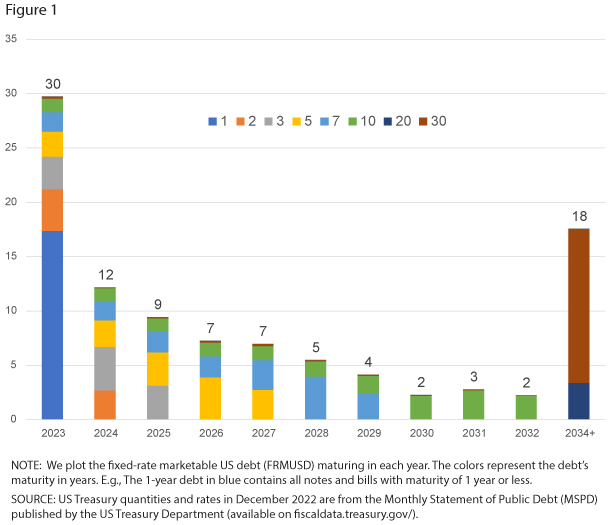
\includegraphics[width=0.55\textwidth]{maturyity.jpg}
        \caption{Source: \href{https://research.stlouisfed.org/publications/economic-synopses/2023/06/02/assessing-the-costs-of-rolling-over-government-debt}{here}}
    \end{figure}
\end{frame}

\begin{frame}{Lessons from the literature}

    \begin{itemize}
        \item State contingent debt and full commitment: \alr{maturity structure irrelevant}
        \item It matters without full commitment (see the dicusssion in Lucas and Stokey (1983)).
        \item The government wanted to smooth tax distortions over time and across states.
        \item We saw an example with complete markets: tax distortions are the same in all states and time periods.
        \item Angeletos (2002): without complete markets but with multiple maturities the government will try to do the same thing. 
    \end{itemize}
\end{frame}



\begin{frame}
    \heading{Maturity determination}
\end{frame}

\begin{frame}{Notation}

    \begin{itemize}
        \item Let there be $J>1$ different maturities of risk-free zero coupon real government debt. 
        \item $b^{j}\bp{s^t}$ is bond issued in state $s^t$ that promises to pay one unit of goods in period $t+j$ ($j$ periods from now).
          
        \item The household budget constraint is now \begin{align*}
            c\bp{s^t} + \sum_{j=1}^J p^j\bp{s^t} b^j\bp{s^t} &= \bp{1-\tau\bp{s^t}} w\bp{s^t} \ell\bp{s^t} \\
        & + \sum_{j=0}^J p^j\bp{s^t} b^j\bp{s^{t-1}}.
        \end{align*}
        \item 
    \end{itemize}
\end{frame}

\begin{frame}{Notation}
 \begin{itemize}
    \item We could also write the budget constraint as 
    \begin{align*}
        c_t + \sum_{j=1}^J p^j_t b^j_t &= \bp{1-\tau_t} w_t \ell_t + \sum_{j=0}^J p^j_t b^j_{t-1}
    \end{align*}
    because nothing is state-contingent.
    \item We do not do it because want to be able to compare the result with the complete markets case. 
    \item Recall: our goal is to show that with a rich enough maturity structure we implement the complete markets optimal allocation.
 \end{itemize}

\end{frame}

\begin{frame}{Environment}
    \begin{itemize}
        \item The rest of the economy is as in Lucas and Stokey (1983):
        \begin{itemize}
        \item The representative household maximizes expected utility;
        \item Linear production function that uses labor only;
        \item Government purchases are Markov, with $S$ possible states of the world;
        \end{itemize}
        \item The only other difference is the government budget constraint: 
        \begin{align*}
            g\bp{s^t} +  \sum_{j=0}^J p^j\bp{s^t} b^j\bp{s^{t-1}} &= \tau\bp{s^t} w\bp{s^t} \ell\bp{s^t} \\
        & +   \sum_{j=1}^J p^j\bp{s^t} b^j\bp{s^t}.
        \end{align*}
        
        \end{itemize}

\end{frame}

\begin{frame}{First order conditions}
    \begin{itemize}
        \item We have $p^0\of{s^t} = 1$. 
        \item The other prices are determined by first order conditions of the household.
        
        \begin{align*}
        p^j\of{s^t} = \beta^j \frac{\E \bs{u_c\of{s^{t+j}}\mid s^t}}{u_c\of{s^t}}.
        \end{align*}
        \item Use these in the budget constraint.
        \end{itemize}
\end{frame}

\begin{frame}{Implementability constraint}
        
        \begin{itemize}
            \item The implementability constraint is now
        \begin{align*}  
            &\overbrace{\sum_{i\geq0,s^{t+i}\geq s^t} \beta^i \pi\of{s^{t+i} \mid s^t} \bs{\frac{u_c\of{s^{t+i}}}{u_c\of{s^t}} c\of{s^{t+i}} + \frac{u_\ell\of{s^{t+i}}}{u_c\of{s^t}} \ell\of{s^{t+i}}  }}^{\alr{z\of{s^t}}} &\\ 
            = &\underbrace{\sum_{j=0}^{J-1} \frac{\E \bs{u_c\of{s^{t+j}}\mid s^t}}{u_c\of{s^t}} b^j\of{s^{t-1}}}_{\alb{a\of{s^t}} \cdot \alg{b\of{s^{t-1}}}} \quad \text{ for all } s^t.& 
        \end{align*}
        
        \item We obtained it by substituting the prices into the budget constraint and summing forward.
        \end{itemize}
\end{frame}

\begin{frame}{Implementability constraint}
    \begin{itemize}
        \item Complete markets:
        \begin{align*}
            \sum_{i,s^i} \beta^i \pi\of{s^i} \bs{\frac{u_c\of{s^i}}{u_c\of{s^0}}c\of{s^i} + \frac{u_\ell\of{s^i}}{u_c\of{s^0}} \ell\of{s^i}} = b_0.
        \end{align*}
        \item Incomplete markets:
        \begin{align*}  
            &\sum_{i\geq0,s^{t+i}\geq s^t} \beta^i \pi\of{s^{t+i} \mid s^t} \bs{\frac{u_c\of{s^{t+i}}}{u_c\of{s^t}} c\of{s^{t+i}} + \frac{u_\ell\of{s^{t+i}}}{u_c\of{s^t}} \ell\of{s^{t+i}}  } &\\ 
            = &\sum_{j=0}^{J-1} \frac{\E \bs{u_c\of{s^{t+j}}\mid s^t}}{u_c\of{s^t}} b^j\of{s^{t-1}} \quad \text{ for all } s^t.& 
        \end{align*}
        \item Idea: to find $\alg{b}$ that satisfies the incomplete markets IC with ${c,\ell}$ from the complete markets allocation.
    \end{itemize}
\end{frame}

\begin{frame}{Implementability constraint}
    \begin{itemize}
        \item Suppose we know the complete markets allocation $c\of{s^t},\ell\of{s^t}$. 
        \item Then we know $\alb{a\of{s^t}}$ and $\alr{z\of{s^t}}$.
        \item We just need to find $\alg{b\of{s^{t-1}}}$ such that the implementability constraint holds given these $\alr{z}$ and $\alb{a}$.
        \item If we manage to do so, it means that we can implement the complete markets allocation with the maturity structure we have.
     \end{itemize}
\end{frame}

\begin{frame}{Implementability constraint}
    \begin{itemize}
        \item We have $S$ distinct states and $J$ distinct maturities.
        \item Let $\alr{Z}$ be a $S \times 1$ vector of $\alr{z\of{s^t}}$, $\alb{A}$ be a $S \times J$ matrix of $\alb{a\of{s^t}}$ and $\alg{B}$ be a $J \times 1$ vector $\alg{b\of{s^{t-1}}}$.
        \item Notice that $\alb{A}$ is a matrix of prices of bonds: $J$ types of bonds in $S$ number of states.
        \item The implementability constraint is \begin{align*} \alr{Z} = \alb{A} \cdot \alg{B}.\end{align*}
    \end{itemize}
\end{frame}

\begin{frame}{Implementing complete markets allocation}
    \begin{itemize}
        \item Pick $\alr{Z}$ and $\alb{A}$ from the complete markets allocation. 
            \item We need to find $\alg{B}$ such that $\alr{Z} = \alb{A} \cdot \alg{B}$. It has to be true for all $s^t$ and $t\geq 0$.
        \item For example: it requires that we can \al{invert} $A$ -- this suggest that, among other things, $J = S$ (otherwise it is not square).
        \item With $J>S$: more than one solution. 
        \item Angeletos (2002): if the number of maturities is at least as large as the number of states, then we can always get \al{arbitrarily close} to complete
        market allocation.
        \item Formally: see Angeletos (2002) for details (and a rigorous proof)

    \end{itemize}
\end{frame}

\begin{frame}
    \heading{Predictions for the maturity structure}
\end{frame}

\begin{frame}{Example}
    \begin{itemize}
        \item Suppose there are two i.i.d. states (L and H) with $g_H > g_L = 0$
        \item Assume there are: two maturities - short (1 period) and long (2 periods). 
        \item Let $b_0 = 0$.
        \item From Lucas and Stokey (1983) we know that with complete markets there is $z_t\of{g_H} =z_H, z_t\of{g_L}=z_L$ with $z_L >  z_H $. 
        \item Normalize $z_H =0$. 
    \end{itemize}
\end{frame}

\begin{frame}{Example}
    \begin{itemize}
        \item We have to solve 
        \begin{align*}
            \left[\begin{array}{c}
            0\\
            z_{L}
            \end{array}\right] & =\left[\begin{array}{cc}
            1 & \beta \frac{\E u_c}{u_c\of{g_H}}\\
            1 & \beta \frac{\E u_c}{u_c\of{g_L}}
            \end{array}\right]\left[\begin{array}{c}
            b^1\\
            b^2\\
            \end{array}\right]
            \end{align*}
        \item This can be inverted as long as $u_c\of{g_H}\neq u_c\of{g_L}$ (otherwise the matrix is singular).
        \item Even if $u_c\of{g_H}=u_c\of{g_L}$, we can still get arbitrarily close to the complete markets allocation -- just set taxes to be slightly different than with complete markets.
    \end{itemize}
\end{frame}

\begin{frame}{Example}
    \begin{itemize}
        \item Usually we have 
        \begin{align*}
            u_c \of{g_L} < u_c \of{g_H}
        \end{align*}
        either due to difference in consumption or labor supply. 
        \item Therefore 
        \begin{align*}
            \det{A} = \beta \frac{\E u_c}{u_c\of{g_H} u_c\of{g_L}} \bs{u_c\of{g_H}-u_c\of{g_L}} > 0.
        \end{align*}
        and the optimal debt porfolio is 
        \begin{align*} 
            \left[\begin{array}{c}
                b^1\\
                b^2\\
                \end{array}\right]                  =
                \frac{z_L}{\det{A}}
                \left[\begin{array}{c}
                -u_c \of{g_L} \E u_c\\
                1\\
                \end{array}\right] 
        \end{align*}
     \end{itemize}
\end{frame}

\begin{frame}{Example}
    \begin{itemize}
        \item In this example $b^1 < 0$ and $b^2 > 0$. 
        \item The government \al{buys} the short maturity debt and \al{sells} the long maturity debt.
        \item Reserve fund financed by long-term debt.
        \item Intuition: in states with high government purchases the value of portfolio \alg{increases} (short term debt becomes cheaper relative to long term debt).
        \item Short term interest rates increase by more than long term interest rates $\rightarrow$ government gets extra income from this portfolio 
        \item What determines the optimal size of portfolio? 
    \end{itemize}
\end{frame}

\begin{frame}{Optimal portfolio size}
    \begin{itemize}
        \item Notice that if  $\det{A}$ is small, then the optimal portfolio size is large.
        \item $\det{A}$ is small if $u_c\of{g_H}-u_c\of{g_L}$ is small -- if marginal utility of consumption is similar in both states.
        \item Variance of consumption in the data is small.
        \item This approach suggests \alr{very large} portfolio sizes!
    \end{itemize}
\end{frame}

\begin{frame}{Buera and Nicolini (2004)}
    \begin{figure}
        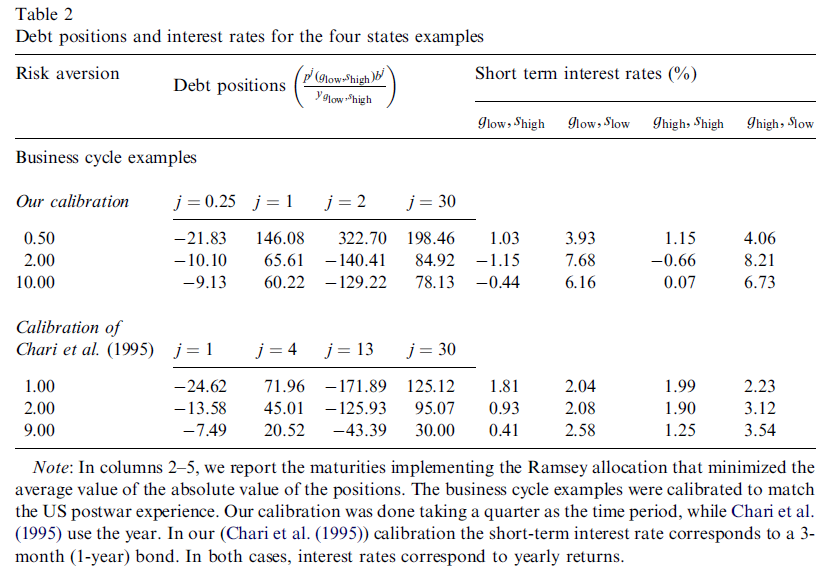
\includegraphics[width=0.7\textwidth]{bueranicolini.png}
    \end{figure}
\end{frame}

\begin{frame}{What is driving this result?}
    \begin{itemize}
        \item We can rewrite the system of equations as 
        \begin{align*}
            \left[\begin{array}{c}
            0\\
            z_{L}
            \end{array}\right] & =\left[\begin{array}{cc}
            1 & R_L ^{-1}\\
            1 & R_H ^{-1} \\
            \end{array}\right]\left[\begin{array}{c}
            b^1\\
            b^2\\
            \end{array}\right]
            \end{align*}
        where we simply used the fact that short-term interest rates satisfy $1 = \beta R_X \frac{\E u_c}{u_c\of{g_X}}$.
        \item These returns are perfectly correlated with shocks (high when $g$ is high) and their volatility is the same as the volatility of $u_c$.
        \item Since the volatility of $u_c$ is small, the volatility of short-term returns is small. 
        \item Buying short-term debt is a \alb{good hedge} against shocks, the risk is very small. Issue long-term debt to finance it!
    \end{itemize}
\end{frame}

\begin{frame}{Problems...}
    \begin{itemize}
        \item Is it true that returns on short-term debt are perfectly correlated with shocks in the data?
        \item Is it true that their volatility is the same as the volatility of $u_c$?
        \item \alr{No.}
    \end{itemize}
\end{frame}

\begin{frame}{Problems...}
    \begin{itemize}
        \item In the data returns are very weakly correlated with consumption growth. 
        \item Suppose we estimate \begin{align*}
            \ln c_{t+1} - \ln c_t = \alpha_0 + \alpha_1 R_t + e_t
        \end{align*}
        \item In our model $\alpha_1 \approx 1$.
        \item In the data $\alpha_1 \approx 0$. 
    \end{itemize}
\end{frame}

\begin{frame}{Problems...}
    \begin{figure}
        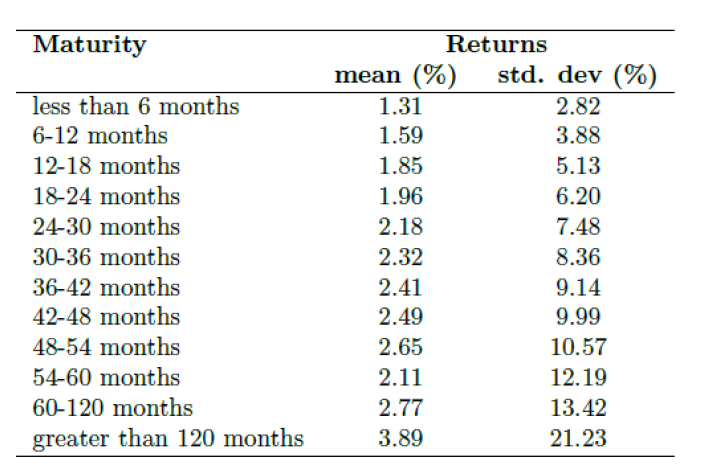
\includegraphics[width=0.65\textwidth]{returns.png}
    \end{figure}
    \begin{itemize}
        \item Volatility of returns is high.
        \item Standard deviation of $\ln c_t$ is around 1\% -- much lower than the volatility of returns...
    \end{itemize}
\end{frame}

\begin{frame}{Summary}
    \begin{itemize}
        \item Portolio suggested by Angeletos (2002) and Buera and Nicolini (2004) is \alr{bad} given the data.
        \item It would be very risky for the government. 
        \item We do not see anything resembling this porfolio in the data!
        \item The problem was that this simple model is terrible at explaining asset prices. 
        \item Bhandari et al. in several papers show that with preferences matching asset prices much better the optimal maturity structure is much more reasonable.
    \end{itemize}
\end{frame}

\begin{frame}{BEGS (2017)}
    \begin{figure}
        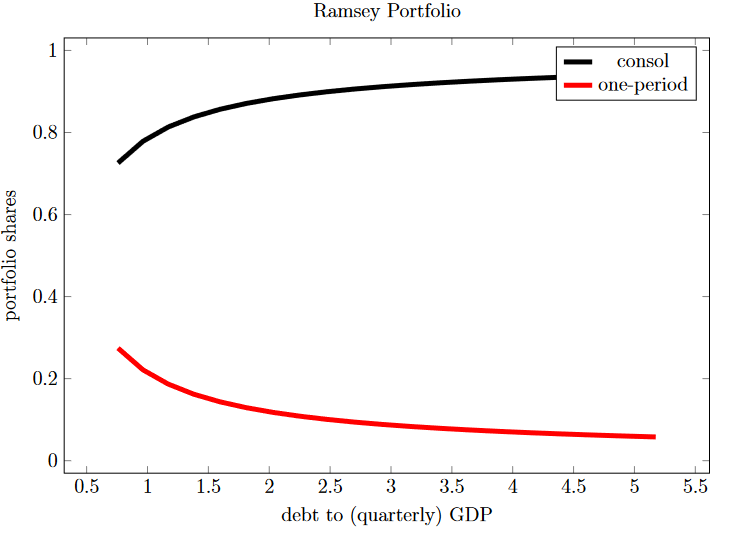
\includegraphics[width=0.5\textwidth]{begs1.png}
        \caption{Source: Bhandari et al. (2017)}
    \end{figure}
\end{frame}

\begin{frame}{BEGS (2017)}
    \begin{figure}
        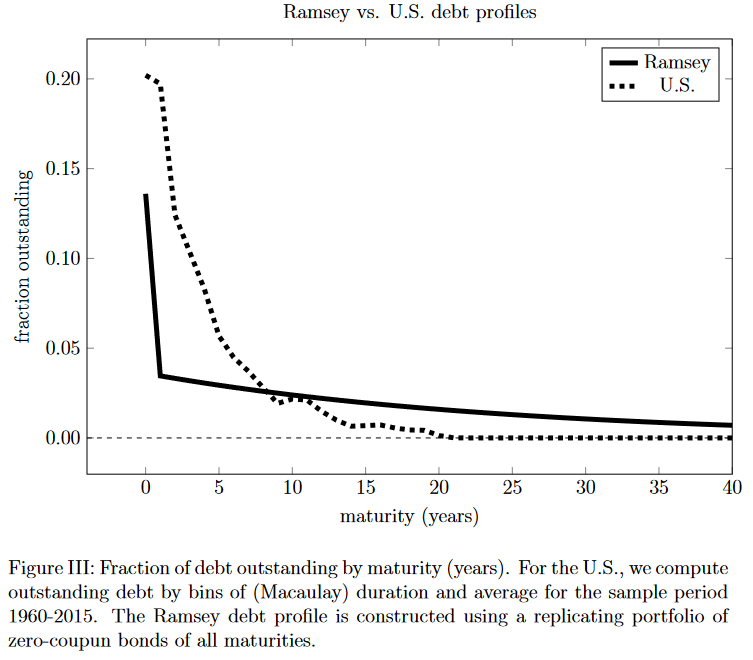
\includegraphics[width=0.5\textwidth]{begs2.png}
        \caption{Source: Bhandari et al. (2017)}
    \end{figure}
\end{frame}

\begin{frame}{BEGS (2017)}
    \begin{figure}
        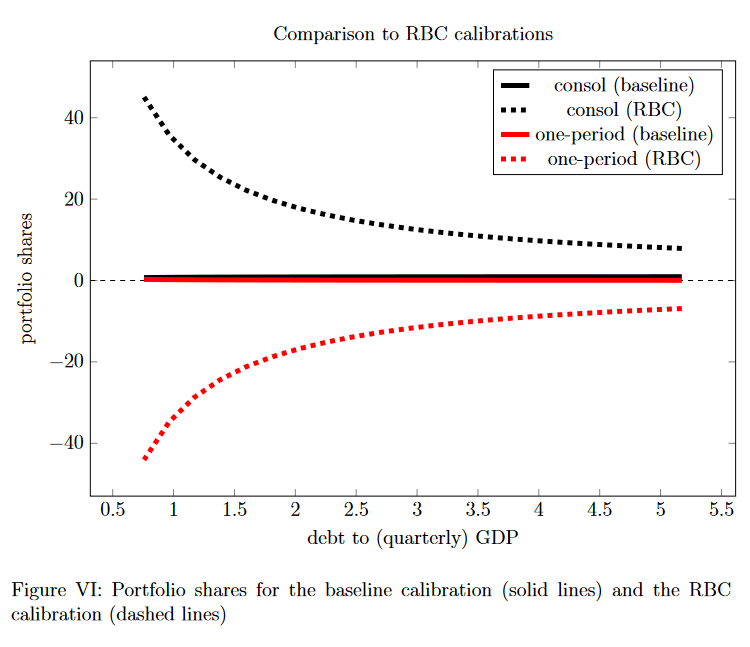
\includegraphics[width=0.5\textwidth]{begs3.png}
        \caption{Source: Bhandari et al. (2017)}
    \end{figure}
\end{frame}

\end{document}